\documentclass[8pt]{beamer}



\mode<presentation>
{
%  \usetheme{Berkeley}
	\usetheme{Dresden}
%	\usetheme{Berlin}
%   \usecolortheme{dove}
%   \usecolortheme{dolphin}
%   \useinnertheme{circles}
   
  \setbeamercovered{transparent}

}


\usepackage[english]{babel}
\usepackage[utf8]{inputenc}
\usepackage{times}
\usepackage[T1]{fontenc}
\usepackage{multimedia}
\usepackage[absolute,overlay]{textpos}
\usepackage{graphicx}

\usepackage{xcolor}
\usepackage{amsmath}
\usepackage[absolute,overlay]{textpos}
\usepackage{physics}
\usepackage{fixltx2e}

\graphicspath{{./media/images/}}

\definecolor{paint}{RGB}{150,0,0}
\setbeamercolor {structure} {fg=paint}
%\setbeamercolor{title}{fg=black}
%\setbeamertemplate{itemize items}[circle]




\newcommand{\jsqrt}[2]{\bqty{ #1 #1 | #2 #2 }}
\newcommand{\ksqrt}[2]{\bqty{ #1 #2 | #2 #1 }}
\newcommand\mf[1]{\mathbf{#1}}
\newcommand\dens{\rho(\mathbf{r})}
\newcommand\densin{\rho^{in}(\mathbf{r})}
\newcommand\densout{\rho^{out}(\mathbf{r})}
\newcommand\rdens{\tilde{\rho}(\mathbf{G})}
\newcommand\erre{\mathbf{r}}
\newcommand\GI{\mathbf{G}}
\newcommand\QE{\textsc{Quantum} ESPRESSO }
\newcommand\numbands{n_{bands}}
\newcommand\numG{n_{G}}
\newcommand\numR{n_{R}}
\newcommand\bigO{\mathcal{O}}
\newcommand\CO{Co\textsubscript{3}O\textsubscript{4} } 


\title[Tuning the computational architecture for Quantum Espresso ab initio calculation of nanostructures] % (optional, use only with long paper titles)
{Tuning the computational architecture for Quantum Espresso ab initio calculation of nanostructures}

\author[Giorgio Ruffa] 
{Giorgio Ruffa}
\institute[Università degli Studi di Milano]{Università degli Studi di Milano}

\date{28 Aprile 2016} 

\subject{}


\begin{document}

% ********** 1 slide *****************
\begin{frame}
  \titlepage
\end{frame}

\section{Introduzione}
\subsection{\QE e la Density Functional Theory}
% ********** slide 2 *****************

\begin{frame}{Introduzione}
\begin{center}
		
\includegraphics[width=4cm]{beam_qe_logo.jpg}
\end{center}
\begin{columns}
	\column{0.33\textwidth}
		\begin{center}
			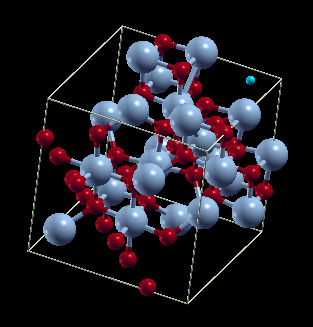
\includegraphics[height=3.5cm]{beam_co3.png}
		\end{center}
	\column{0.33\textwidth}
		\begin{center}
			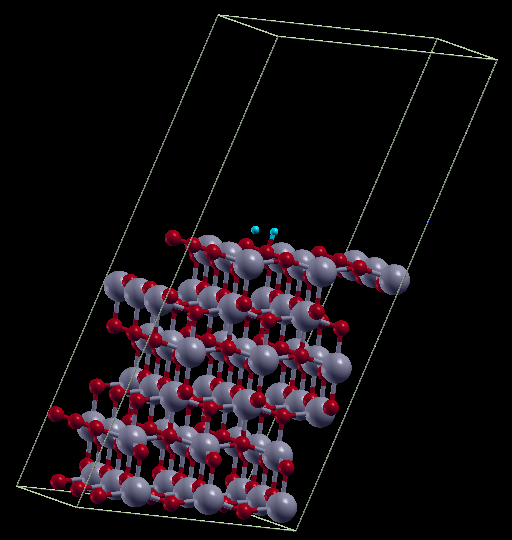
\includegraphics[height=3.5cm]{titania_crystal.png}
		\end{center}
	\column{0.33\textwidth}
		\begin{center}
			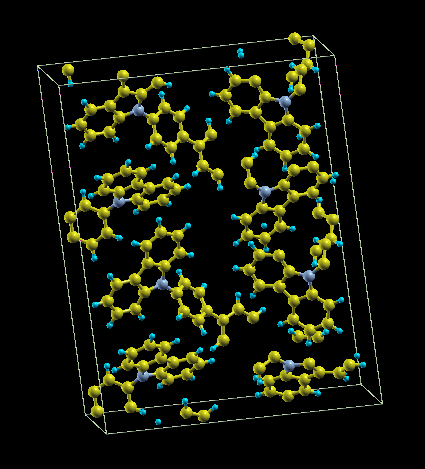
\includegraphics[height=3.5cm]{beam_cbp.png}
		\end{center}
\end{columns}
		
\end{frame}

% ********** slide 3 *****************
\begin{frame}{Introduzione}


\begin{columns}
	\column{0.5\textwidth}
%		\begin{center}
%			
\includegraphics[width=4cm]{beam_qe_logo.jpg}		
%		\end{center}
	
	\invisible<1>{\begin{block}{Density Functional Theory (DFT)}
		\begin{itemize}
			\setlength\itemsep{1em}
			\item[]<2-> Equazioni di Kohn-Sham :
			\item[]<2-> $ \displaystyle  \lbrace  - \frac{1}{2} \nabla^2+ v_{eff}(\erre) \rbrace 	\psi_{j}^{KS}(\erre) = \varepsilon_{j}^{KS} 	\psi_{j}^{KS}(\erre)$
			\item[]<3-> $ \displaystyle  v_{eff}(\erre) = v_{ion}(\erre) + v_{h}(\erre) + v_{xc}(\erre)$
			\item[]<3-> $ \displaystyle v_{h}(\erre) = \int \frac{\rho(\erre')}{\mid \erre - \erre'\mid} \dd{\erre'} $
			\item[]<3-> $ \displaystyle v_{xc}(\erre) =	\frac{\var{E_{xc}[\dens]}}{\var{\dens}}$
		\end{itemize}
	\end{block}}
		
	\column{0.5\textwidth}
		\begin{center}

			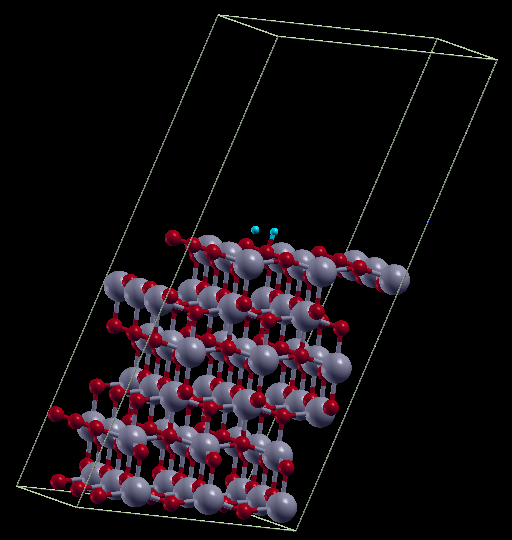
\includegraphics[width=3.5cm]{titania_crystal.png}	\\

			~ \\
			Superficie TiO\textsubscript{2} : \\ $ 150$ Atomi $\sim 2 \cdot 10 ^{3} e^{-}$	

		\end{center}
\end{columns}

\end{frame}

% ********** slide 4 *****************
\begin{frame}{Self Consistent DFT}
\begin{center}
	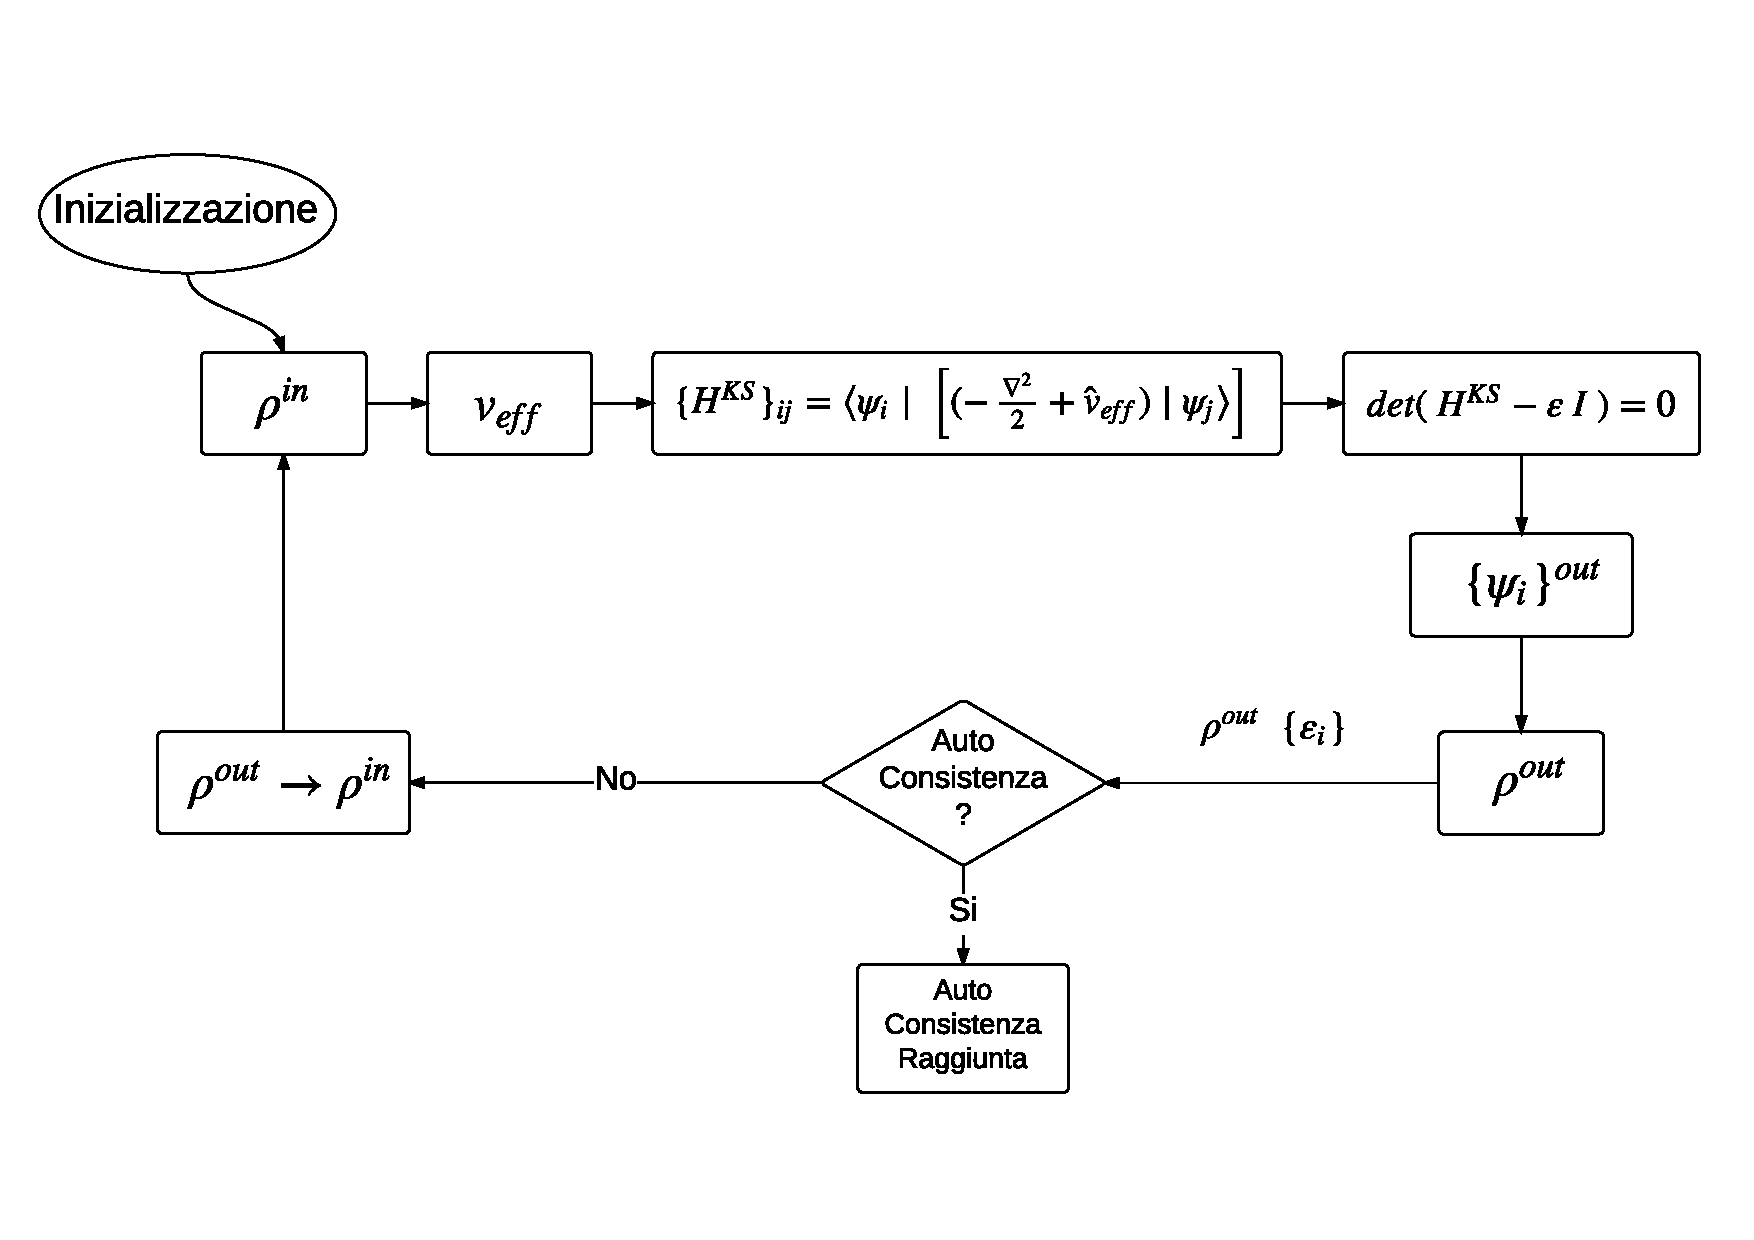
\includegraphics[width=\textwidth]{beam_SCF_0.pdf}	
\end{center}
\end{frame}



% ********** slide 5 *****************
\begin{frame}{Self Consistent}
\begin{center}
	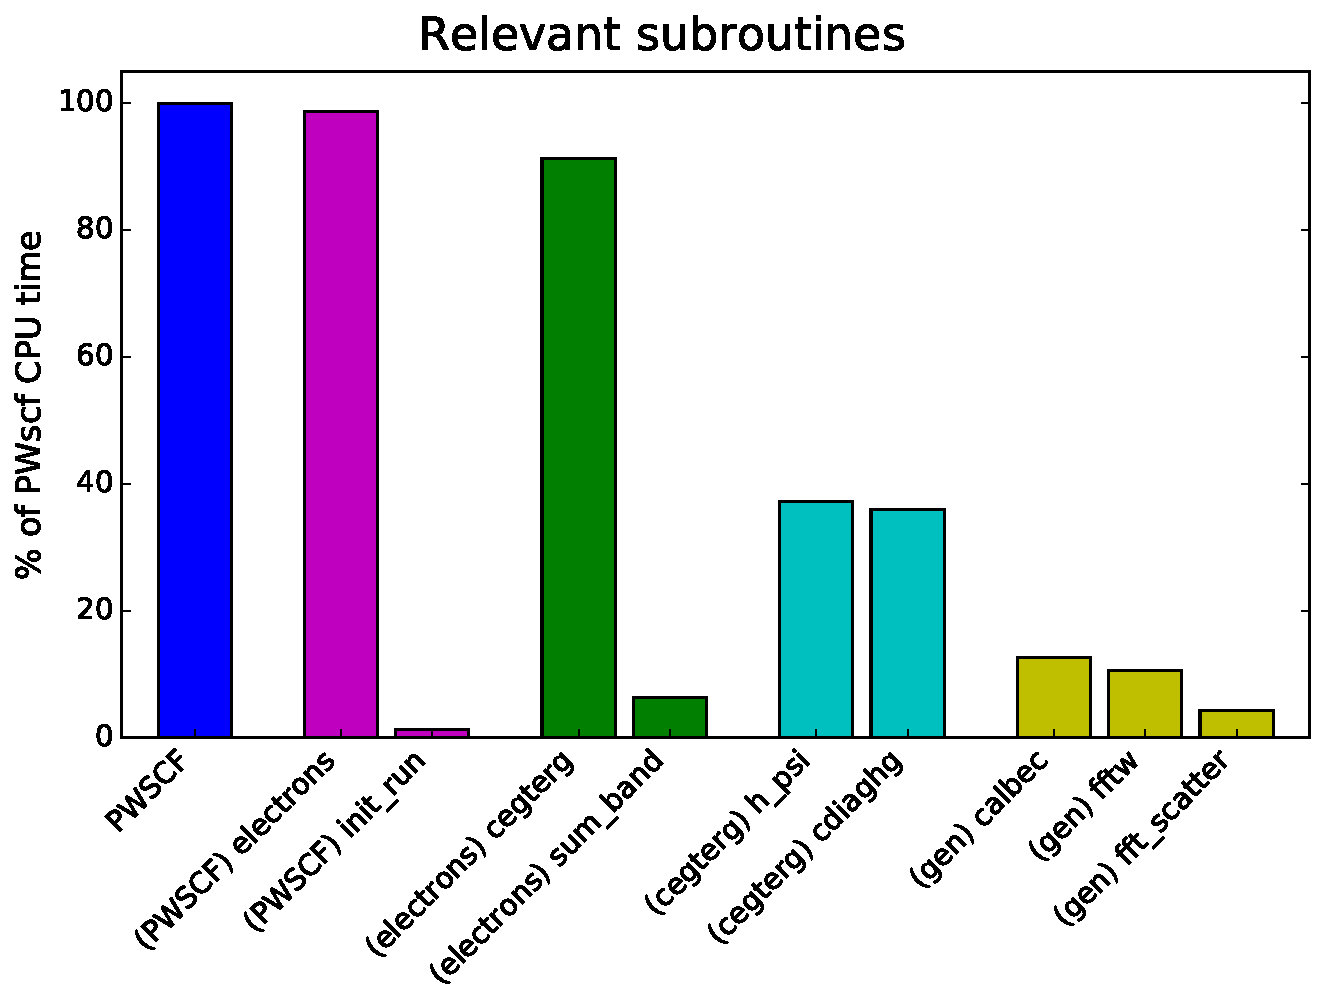
\includegraphics[width=\textheight]{beam_relevant_subroutines.pdf}	
\end{center}
\end{frame}



\end{document}
